\documentclass[titlepage,a4paper,12pt]{report}
\usepackage{amssymb,amsfonts,amsmath}
\usepackage{fullpage}
\usepackage{graphicx}
%\usepackage[cc]{titlepic}
\usepackage{amsthm}
\newtheorem{definition}{Definition}[section]
\newtheorem{example}{Example}[section]
\newtheorem{theorem}{Theorem}[section]
\newtheorem{exercise}{Exercise}[section]
\newtheorem{corollary}{Corollary}[section]
\newtheorem{proposition}{Proposition}[section]
\pdfpagewidth 8.5in
\pdfpageheight 11in
\setlength\topmargin{-0.5in}
\setlength\headheight{0in}
\setlength\headsep{0in}
\setlength\textheight{9.5in}
\setlength\textwidth{7.0in}
\setlength\oddsidemargin{-0.5in}
\setlength\evensidemargin{1.0in}
\setlength\parindent{0.25in}
\setlength\parskip{0.25in}
%\begin{titlepage}
%\usepackage{titlepic}
%\titlepic{
\includegraphics[width=0.2\textwidth]{uz1.png}}
%
%\title{\textbf{HMTH111 Calculus 2}}
%\author{Nhawu. G\\
%		Department of Mathematics\\
%		University of Zimbabwe, ZIM}
%
%\end{titlepage}

\begin{document}
\begin{titlepage}
 
\begin{center}
 
 
% Upper part of the page

\includegraphics[width=0.15\textwidth]{uz1.png}\\[1cm]
 
\textsc{\LARGE University of Zimbabwe}\\[1.5cm]
 
\textsc{\Large HMTHCS111 CALCULUS 2}\\[0.5cm]
 
 
% Title

{ \huge \bfseries Calculus of Several Variables}\\[0.4cm]
 

 
% Author and supervisor
\begin{minipage}{0.4\textwidth}
\begin{center} \large
\emph{Author:}\\
G. \textsc{Nhawu}
\end{center}
\end{minipage}
\begin{minipage}{0.4\textwidth}
\begin{flushright} \large
\emph{Department:} \\
\textsc{Mathematics and Computational Sciences}
\end{flushright}
\end{minipage}

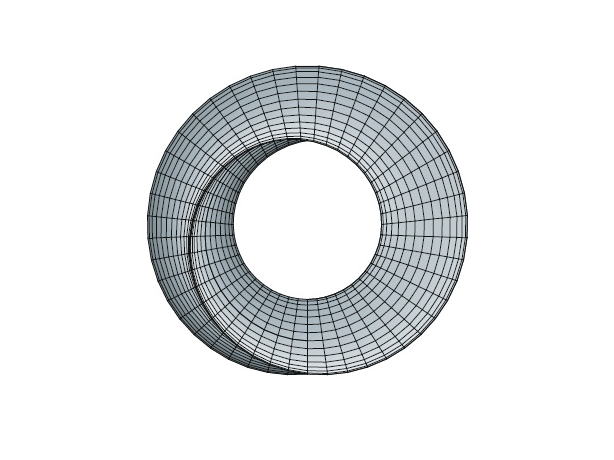
\includegraphics[width=0.7\textwidth]{umblictorus.png}\\[1cm]
 \vfill
 
 
% Bottom of the page
{\large \today}
 
\end{center}
 
\end{titlepage}
%\maketitle
\tableofcontents
\setcounter{chapter}{6}
\chapter{Multiple Integration}
\begin{center}
\small{\parbox{18cm}{
		\begin{raggedright}
		{\small
		\textit{There was a young man from Trinity,
Who solved the square root of infinity.
While counting the digits,
He was seized by the fidgets,
Dropped science, and took up divinity.}
 }
 
				\vspace{.5cm}\hfill{---Author Unknown}
		\end{raggedright}
	}
} 
\end{center}
\section{Iterated Integrals}
In the previous chapter, we saw that it is meaningful to differentiate functions of several variables with respect to one variable while holding the other variable constant, we can integrate functions of several variables by a similar procedure. For example, if we have the partial derivative\\ $f_x(x,y)=2xy$, then by considering $y$ constant, we can integrate with respect to $x$ to obtain 
\begin{eqnarray*}
f(x,y) &=& \int f_x(x,y)\, dx  \quad ~~~~~~~~ \mbox{Integrate with respect to $x$} \\
&=& \int 2xy \, dx  \quad ~~~~~~~~~~~~~\mbox{$y$ is held constant}\\
&=& y\int 2x\, dx \quad ~~~~~~~~~~~~~ \mbox{Factor out constant $y$} \\
&=&y(x^2)+C(y) \quad ~~~~~~~~ \mbox{Anti-derivative of $2x$ is $x^2$}\\
&=& x^2+C(y). \quad ~~~~~~~~~~~\mbox{$C(y)$ is function of $y$}
\end{eqnarray*}
Note that the constant of integration, $C(y)$ is a function of $y$. In other words, by integrating with respect to $x$, we are able to recover $f(x,y)$ only partially. For example, by considering $y$ constant, we can apply the Fundamental Theorem of calculus to evaluate 
\[\int _1 ^{2y} 2xy\, dx =x^2y \Biggl |_1^{2y}=(2y)^2y-(1)^2y=4y^3-y.\]
Note that the variable of integration cannot appear in either limit of integration. For example, it makes no sense to write $\displaystyle \int _0^x y\, dx$.
\begin{example}
Evaluate $\displaystyle \int _1^x (2x^2y^{-2}+2y)\, dy$.

\noindent \textbf{Solution:} Considering $x$ to be constant and integrating with respect to $y$ produces 
\begin{eqnarray*}
\int _1^x (2x^2y^{-2}+2y)\, dy &=& \left[\dfrac{-2x^2}{y}+y^2\right] _1^x \\
&=& \left(\dfrac{-2x^2}{x}+x^2\right)-\left(\dfrac{-2x^2}{1}+1\right)\\
&=& 3x^2-2x-1.
\end{eqnarray*}
\end{example}
\noindent Notice that in the above example the integral defines a function of $x$ and can \textit{itself} be integrated.
\begin{example}
Evaluate $\displaystyle \int _1^2\left[ \int _1^x (2x^2y^{-2}+2y)\, dy\right]\, dx$.

\noindent \textbf{Solution:}
\begin{figure}[h!]
\input{int.pic}
\caption{The region of integration}
\end{figure}

 Using the result from the previous example, we have 
\begin{eqnarray*}
\int _1^2\left[ \int _1^x (2x^2y^{-2}+2y)\, dy\right]\, dx &=& \int _1^2 (3x^2-2x-1)\, dx\\
&=& \left[ x^3-x^2-x\right]_1^2 \\
&=& 2-(-1)\\
&=& 3.
\end{eqnarray*} 
\end{example}
\noindent The integral in the above example is an \textbf{iterated integral}. Iterated integrals are usually written simply as 
\[\int _a^b \int _{g_1(x)}^{g_2(x)}f(x,y)\, dydx \quad \mbox{and} \quad \int _c^d \int _{h_1(y)}^{h_2(y)}f(x,y)\, dxdy.\]
The \textbf{inside limits of integration} can be variable with respect to the outer variable of integration. However, the \textbf{outside limits of integration} must be constant with respect to both variables of integration. After performing the inside integration, we obtain a definite integral, and the second integration produces a real number.

\noindent One order of integration will often produce a simpler integration problem than the other order. The order of integration affects the ease of integration, but not the value of the integral.

\subsection{Comparing Different Orders of Integration}
\begin{example}
Sketch the region whose area is represented by the integral 
\[\int _0^2 \int _{y^2}^4 dxdy.\]
Then find another iterated integral using the order $dydx$ to represent the area, and show that both integrals yield the same value.

\noindent \textbf{Solution:} 
\begin{figure}[ht!]
\input{int2.pic}
\caption{Fig 1}
\end{figure} 
From the given limits of integration, we know that 
\[y^2\leq x\leq 4 \quad \mbox{Inner limits of integration}\] which means that the region $R$ is bounded on the left by the parabola $x=y^2$ and on the right by the line $x=4$. Furthermore, because
\[0 \leq y \leq 2 \quad \mbox{Outer limits of integration}\] we know that $R$ bounded below by the $x$-axis. 
The value of this integral is 
\begin{eqnarray*}
\int _0^2 \int _{y^2}^4 dxdy &=& \int _0^2 x \Biggl ]_{y^2}^4 dy \\
&=& \int _0^2 (4-y^2)\, dy \\
&=& \left[ 4y-\dfrac{y^3}{3}\right]_0^2 =\dfrac{16}{3}.
\end{eqnarray*}
To change the order of integration to $dydx$, place a vertical rectangle in the region. From this we can see that the constant bounds $0\leq x \leq 4$ serve as the outer limits of integration. By solving for $y$ in the equation $x=y^2$, we can conclude that the inner bounds are $0\leq y \leq \sqrt{x}$. Therefore, the area of the region can be represented by 
\[\int _0^4 \int _0^{\sqrt{x}} dydx.\]
\begin{figure}[ht!]
\input{int3.pic}
\caption{Fig 2}
\end{figure}
By evaluating this integral, we can see that it has the same value as the original integral.
\begin{eqnarray*}
\int _0^4 \int _0^{\sqrt{x}} dydx &=& \int _0^4 y\Biggl ]_0^{\sqrt{x}} dx \\
&=& \int _0^4 \sqrt{x}\, dx \\
&=& \dfrac{2}{3}x^{\frac{3}{2}}\Biggl ]_0^4 =\dfrac{16}{3}.
\end{eqnarray*}
\end{example}
\begin{example}
Express $\displaystyle \int _0^4\int _{\frac{x}{2}}^2 e^{y^2}\, dydx$ as an iterated integral with order of integration reversed and evaluate.

\noindent \textbf{Solution:} From the given limits of integration we see that, for a fixed $x$, $y$ varies from $y=\frac{x}{2}$ to $y=2$ and $x$ varies from $x=0$ to $x=4$. We can also describe the region as, for $y$ fixed, $x$ varies from $x=0$ to $x=2y$ and $y$ varies from $y=0$ to $y=2$. The corresponding iterated integral is $\displaystyle \int _0^2\int _0^{2y}e^{y^2}\, dxdy$.
Solving, we have
\begin{eqnarray*}
\int _0^2\int _0^{2y} e^{y^2}\, dxdy &=& \int _0^2xe^{y^2}\biggr]_{x=0}^{x=2y}\, dy \\
&=& \int _0^2 2ye^{y^2}\, dy \\
&=& e^{y^2}\biggr]_0^2 \\
&=& e^4-1.
\end{eqnarray*}
\end{example}
\begin{example}
Evaluate $\displaystyle \int _0^2\int _{\frac{y}{2}}^1 ye^{x^3}\, dxdy$.

\noindent \textbf{Solution:} We cannot integrate first with respect to $x$, as indicated, because it happens that $e^{x^3}$ has no elementary anti-derivative. So we try to evaluate the integral by first reversing the order of integration.
\begin{eqnarray*}
\int _0^2\int _{\frac{y}{2}}^1ye^{x^3}\, dxdy &=& \int _0^1\int _0^{2x}ye^{x^3}\, dydx\\
&=& \int _0^1 \dfrac{1}{2}y^2\biggl]_0^2x e^{x^3}\, dx\\
&=& \int _0^1 2x^2 e^{x^3}\, dx\\
&=& \dfrac{2}{3}e^{x^3}\biggl]_0^1\\
&=& \dfrac{2}{3}(e-1).
\end{eqnarray*}
\end{example}
\section{Double Integrals and Volume}
\subsection{Double Integrals and Volume of a Solid Region}
\subsubsection{Definition of Double Integral}
If $f$ is defined on a closed, bounded region $R$ in the $xy$-plane, then the \textbf{double integral of $f$ over $R$} is given by 
\[\iint \limits _R f(x,y)\, dA =\lim _{|\Delta|\rightarrow 0}\sum _{i=1}^n f(x_i, y_i)\Delta x_i \Delta y_i\] provided the limit exists. If the limit exists, then $f$ is \textbf{integrable} over $R$.

\noindent A double integral can be used to find the volume of a solid region that lies between the $xy$-plane and the surface given by $z=f(x,y)$.
\subsubsection{Volume of a Solid Region}
If $f$ is integrable over a plane region $R$ and $f(x,y)\geq 0$ for all $(x,y)$ in $R$, then the volume of the solid region that lies above $R$ and below the graph of $f$ is defined as 
\[V= \iint \limits _R f(x,y)\, dA.\]
\begin{example}
Find the volume of the solid region $R$ bounded by the surface \[f(x,y)=e^{-x^2}\] and the planes $y=0, y=x$ and $x=1$.

\noindent \textbf{Solution:} The base of $R$ in the $xy$-plane is bounded by the lines $y=0, x=1$ and $y=x$. The two possible orders of integration are 
\[\int _0^1 \int _0^x e^{-x^2}\, dydx \quad \mbox{and} \quad \int _0^1 \int _y^1 e^{-x^2}\, dxdy.\] By setting up the corresponding iterated integrals, we can see that the order $dxdy$ requires the anti-derivative $\displaystyle \int e^{-x^2}\, dx$, which is not an elementary function. On the other hand, the order $dydx$ produces the integral
\begin{eqnarray*}
\int _1^0 \int _0^x e^{-x^2}\, dydx &=& \int _0^1 e^{-x^2}y\Biggl ]_0^x \, dx\\
&=& \int _0^1 xe^{-x^2}\, dx \\
&=& -\dfrac{1}{2}e^{-x^2}\Biggl ]_0^1\\
&=& -\dfrac{1}{2}\left(\dfrac{1}{e}-1\right)\\
&=& \dfrac{e-1}{2e} = 0.316.
\end{eqnarray*} 
\end{example}
\section{Triple Integrals}
\subsubsection{Definition of Triple Integral}
If $f$ is continuous over a bounded solid region $Q$, then the \textbf{triple integral of $f$ over $Q$} is defined as 
\[\iiint \limits _Q f(x,y,z)\, dV=\lim _{|\Delta|\rightarrow 0}\sum _{i=1}^n f(x_i, y_i, z_i)\, \Delta V_i \] provided the limit exists. The \textbf{volume} of the solid region $Q$ is given by 
\[\mbox{Volume of Q} =\iiint \limits _Q dV. \]
\subsubsection{Evaluation by Iterated Integrals}
Let $f$ be continuous on a solid region $Q$ defined by 
\[a\leq x\leq b, \quad h_1(x)\leq y \leq h_2(x), \quad g_1(x,y)\leq z \leq g_2(x,y)\] where $h_1, h_2, g_1$ and $g_2$ are continuous functions. Then 
\[\iiint \limits_Q f(x,y,z)\, dV =\int _a^b \int _{h_1(x)}^{h_2(x)}\int _{g_1(x,y)}^{g_2(x,y)}f(x,y,z)\, dV.\]
\begin{example}
Evaluate the triple iterated integral 
\[\int _0^2 \int _0^x \int _0^{x+y}e^x(y+2z)\, dzdydx.\]

\noindent \textbf{Solution:} For the first integration, hold $x$ and $y$ constant and integrate with respect to $z$. 
\begin{eqnarray*}
\int _0^2 \int _0^x \int _0^{x+y}e^x(y+2z)\, dzdydx &=& \int _0^2\int _0^x e^x(yz+z^2)\Biggl ]_0^{x+y} \, dydx \\
&=& \int _0^2 \int _0^x e^x(x^2+3xy+2y^2)\, dydx.
\end{eqnarray*}
For the second integration, hold $x$ constant and integrate with respect to $y$.
\begin{eqnarray*}
\int _0^2 \int _0^x e^x(x^2+3xy+2y^2)\, dydx &=& \int _0^2 \left[ e^x\left(x^2y+\dfrac{3xy^2}{2}+\dfrac{2y^3}{3}\right)\right]_0^x \, dx \\
&=& \dfrac{19}{6}\int _0^2 x^3e^x\, dx \\
&=& \dfrac{19}{6}\Biggl[e^x(x^3-3x^2+6x-6)\Biggr]_0^2 \\
&=& \dfrac{19}{6}\left(\dfrac{e^2}{3}+1\right).
\end{eqnarray*}
\end{example}
\begin{example}
If $f(x,y,z)=xy+yz$ and $T$ consists of those points $(x,y,z)$ in space satisfying the inequalities $-1\leq x\leq 1, \, 2\leq y\leq 3$ and $0\leq z\leq 1$, then 
\begin{eqnarray*}
\iint \limits _T f(x,y,z)\, dV & =& \int _{-1}^1 \int _2^3\int _0^1 (xy+yz)\, dzdydx\\
&=& \int _{-1}^1\int _2^3 \left[xyz+\dfrac{1}{2}yz^2\right]_{z=0}^1\, dydx\\
&=& \int _{-1}^1\int _2^3 \left(xy+\frac{1}{2}y\right)\, dydx\\
&=& \int _{-1}^1\left[\dfrac{1}{2}xy^2+\dfrac{1}{4}y^2\right]_{y=2}^3\, dx\\
&=& =\int _{-1}^1 \left(\dfrac{5}{2}x+\dfrac{5}{4}\right)\, dx \\
&=& \left[\dfrac{5}{4}x^2+\dfrac{5}{4}x\right]_{-1}^1=\dfrac{5}{2}.
\end{eqnarray*}
\end{example}
\section{Change of Variables : Jacobians}
\subsection{Jacobians}
The Jacobian is named after the German mathematician Carl Gustav Jacobi (1804-1851). For the single integral 
\[\int _a^b f(x)\, dx\] you can change variables by letting $x=g(u)$, so that $dx=g'(u)du$, and obtain 
\[\int _a^b f(x)\, dx = \int _c^d f(g(u))g'(u)\, du\] where $a=g(c)$ and $b=g(d)$. Note that the change of variable introduces an additional factor $g'(u)$ into the integrand. This also occurs in the case of double integrals.
\[\iint \limits _R f(x,y)\, dA =\iint \limits _S f(g(u,v), h(u,v))\underbrace{\left |\dfrac{\partial x}{\partial u}\dfrac{\partial y}{\partial v}-\dfrac{\partial y}{\partial u}\dfrac{\partial x}{\partial v}\right|}_{\mbox{Jacobian}}\, dudv\] where the change of variables $x=g(u,v)$ and $y=h(u,v)$ introduces a factor called the \textbf{Jacobian} of $x$ and $y$ with respect to $u$ and $v$.
\subsubsection{Definition of the Jacobian}
If $x=g(u,v)$ and $y=h(u,v)$, then the \textbf{Jacobian} of $x$ and $y$ with respect to $u$ and $v$, denoted by $\dfrac{\partial (x,y)}{\partial (u,v)}$ is 
\[\dfrac{\partial (x,y)}{\partial (u,v)} =\begin{vmatrix}
\dfrac{\partial x}{\partial u} & \dfrac{\partial x}{\partial v} \\~\\
\dfrac{\partial y}{\partial u} & \dfrac{\partial y}{\partial v}
\end{vmatrix} =\dfrac{\partial x}{\partial u}\dfrac{\partial y}{\partial v}-\dfrac{\partial y}{\partial u}\dfrac{\partial x}{\partial v}. \]
In cases it is more convenient to express $u$ and $v$ in terms of $x$ and $y$, we can first compute $\dfrac{\partial (u,v)}{\partial (x,y)}$ explicitly and then find the needed Jacobian $\dfrac{\partial (x,y)}{\partial (u,v)}$ from the formula
\[\dfrac{\partial (x,y)}{\partial (u,v)}\cdot \dfrac{\partial (u,v)}{\partial (x,y)}=1.\]
\begin{example}
Find the Jacobian for the change of variables defined by 
\[x=r\cos \theta \quad \mbox{and} \quad y=r\sin \theta.\]

\noindent \textbf{Solution:} From the definition of a Jacobian, we obtain 
\[\dfrac{\partial (x,y)}{\partial (r,\theta)} =\begin{vmatrix}
\dfrac{\partial x}{\partial r} & \dfrac{\partial x}{\partial \theta} \\~\\
\dfrac{\partial y}{\partial r} & \dfrac{\partial y}{\partial \theta}
\end{vmatrix}=\begin{vmatrix}
\cos \theta & -r\sin \theta \\
\sin \theta & r\cos \theta
\end{vmatrix} =r\cos ^2 \theta +r\sin ^2 \theta =r.\]
\end{example}
\noindent The above example points out that the change of variables from rectangular to polar coordinates for a double integral can be written as 
\begin{eqnarray*}
\iint \limits _R f(x,y)\, dA &=& \iint \limits _S f(r\cos \theta , r \sin \theta)\, rdrd\theta , r>0 \\
&=& \iint \limits _S f(r\cos \theta , r \sin \theta)\left|\dfrac{\partial (x,y)}{\partial (r, \theta)}\right|\, drd\theta 
\end{eqnarray*}
where $S$ is the region in the $r\theta$-plane that corresponds to the region $R$ in the $xy$-plane. In general, a change of variables is given by a one-to-one \textbf{transformation} $T$ from a region $S$ in the $uv$-plane to a region $R$ in the $xy$-plane, to be given by 
\[T(u,v)=(x,y)=(g(u,x), h(u,v))\] where $g$ and $h$ have continuous first partial derivatives in the region $S$. Note that the point $(u,v)$ lies in $S$ and the point $(x,y)$ lies in $R$. In most cases, we are hunting for a transformation for which the region $S$ is simpler than the region $R$.
\subsubsection{Change of Variables for Double Integrals}
\begin{theorem}
Let $R$ and $S$ be regions in the $xy$- and $uv$-planes that are related by the equations $x=g(u,v)$ and $y=h(u,v)$ such that each point in $R$ is the image of a unique point in $S$. If $f$ is continuous on $R$, $g$ and $h$ have continuous partial derivatives on $S$, and $\dfrac{\partial (x,y)}{\partial (u,v)}$ is non-zero on $S$, then 
\[\iint \limits _R f(x,y)\, dA =\iint \limits _S f(g(u,v), h(u,v))\left|\dfrac{\partial (x,y)}{\partial (u,v)}\right|\, dudv.\] 
\end{theorem} 
\begin{example}
Let $R$ be the region bounded by the lines 
\[x-2y=0, \quad x-2y=-4, \quad x+y=4, \quad \mbox{and} \quad x+y=1.\] Evaluate the double integral 
\[\iint \limits _R 3xy\, dA.\]

\noindent \textbf{Solution:} to begin, let $u=x+y$ and $v=x-2y$. Solving this system of equations for $x$ and $y$ produces $x=\dfrac{1}{3}(2u+v)$ and $y=\dfrac{1}{3}(u-v)$. The partial derivatives of $x$ and $y$ are 
\[\dfrac{\partial x}{\partial u}=\dfrac{2}{3}, \quad \dfrac{\partial x}{\partial v}=\dfrac{1}{3}, \quad \dfrac{\partial y}{\partial u}=\dfrac{1}{3}\quad \mbox{and} \quad \dfrac{\partial y}{\partial v}=-\dfrac{1}{3}\] which implies that the Jacobian is 
\begin{eqnarray*}
\dfrac{\partial (x,y)}{\partial (u,v)} &=&\begin{vmatrix}
\dfrac{\partial x}{\partial u} & \dfrac{\partial x}{\partial v}\\~\\
\dfrac{\partial y}{\partial u} & \dfrac{\partial y}{\partial v}
\end{vmatrix} \\
&=& \begin{vmatrix}
\dfrac{2}{3} & \dfrac{1}{3} \\~\\
\dfrac{1}{3} & -\dfrac{1}{3}
\end{vmatrix} \\
&=& -\dfrac{2}{9}-\dfrac{1}{9}=-\dfrac{1}{3}.
\end{eqnarray*} 
Therefore, we obtain 
\begin{eqnarray*}
\iint \limits _R 3xy\, dA &=& \iint \limits _S 3\left[\dfrac{1}{3}(2u+v)\dfrac{1}{3}(u-v)\right]\left|\dfrac{\partial (x,y)}{\partial (u,v)}\right|\, dvdu\\
&=& \int _1^4 \int _{-4}^0 \dfrac{1}{9} (2u^2-uv-v^2)\, dvdu\\
&=& \dfrac{1}{9}\int _1^4 \left[ 2u^2v-\dfrac{uv^2}{2}-\dfrac{v^3}{3}\right]_{-4}^0\, du\\
&=& \dfrac{1}{9}\int _1^4 \left(8u^2+8u-\dfrac{64}{3}\right)\, du \\
&=&\dfrac{1}{9}\left[\dfrac{8u^3}{3}+4u^2-\dfrac{64}{3}u\right]_1^4 \\
&=&\dfrac{164}{9}.
\end{eqnarray*}
\end{example}
\begin{example}
Suppose $R$ is the plane bounded by the hyperbolas $xy=1, \, xy=3$ and \\ $x^2-y^2=1, \, x^2=y^2=4$. Find $\displaystyle \iint \limits _R (x^2+y^2)\, dxdy$.

\noindent \textbf{Solution:} The hyperbolas bounding $R$ are $u-$curves and $v-$curves if $u=xy$ and $v=x^2-y^2$.  We can most easily write $x^2+y^2$ in terms of $u$ and $v$ by first noting that \[4u^2+v^2=4x^2y^2+(x^2-y^2)^2=(x^2+y^2)^2,\] so that $x^2+y^2=\sqrt{4u^2+v^2}$. Now 
\[\dfrac{\partial (u,v)}{\partial (x,y)}=\begin{vmatrix}
y & x \\
2x & -2y 
\end{vmatrix}=-2(x^2+y^2).\]
Hence we have 
\[\dfrac{\partial (x,y)}{\partial (u,v)}=-\dfrac{1}{2(x^2+y^2)}=-\dfrac{1}{2\sqrt{4u^2+v^2}}.\]
Therefore
\[\iint \limits _R (x^2+y^2)\, dxdy =\int _1^4\int _1^3 \sqrt{4u^2+v^2}\dfrac{1}{2\sqrt{4u^2+v^2}}\, dudv=\int _1^4\int _1^3\dfrac{1}{2}\, dudv=3.\] 
\end{example}
\begin{example}
Find the area of the region $R$ bounded by the curves $xy=1, \, xy=3$ and\\ $xy^{1.4}=1, \, xy^{1.4}=2$.

\noindent \textbf{Solution:} Define change of variables transformation by $u=xy$ and $v=xy^{1.4}$. Then 
\[\dfrac{\partial (u,v)}{\partial (x,y)}=\begin{vmatrix}
y & x \\
y^{1.4} & (1.4)xy^{0.4}
\end{vmatrix}=(0.4)xy^{1.4}=(0.4)v.\] So $\dfrac{\partial (x,y)}{\partial (u,v)}=\dfrac{1}{\dfrac{\partial (u,v)}{\partial (x,y)}}=\dfrac{2.5}{v}$. Consequently, 
\[\iint \limits _R dxdy =\int _1^2\int _1^3 \dfrac{2.5}{v}\, dudv=5\ln 2.\]
\end{example}
\section{Tutorial Questions}
\begin{enumerate}
\item Evaluate the integral.\\
(i)\, $\displaystyle \int _0^x (2x-y)\, dy$ \quad (ii)\, $\displaystyle \int _x^{x^2} \dfrac{y}{x}\, dy$ \quad (iii)\,  $\displaystyle \int _{e^y}^y \dfrac{y\ln x}{x}\, dx$ \quad (iv)\, $\displaystyle \int _0^{x^3} ye^{-\frac{y}{x}}\, dy$ \quad (v)\, $\displaystyle \int _0^{\cos x} y\, dy$.
\item Evaluate the iterated integral.\\
(i)\, $\displaystyle \int _0^1\int _0^2 (x+y)\, dydx$ \quad (ii)\, $\displaystyle \int _0^1\int _0^x \sqrt{1-x^2}\, dydx$ \quad (iii)\,$\displaystyle \int _0^2\int _{3y^2-6y}^{2y-y^2} 3y\, dxdy$ \quad (iv)\, $\displaystyle \int _0^{\frac{\pi}{2}}\int _0^{\sin \theta} \theta r\, drd\theta$.
\item Sketch the region $R$ of integration and switch the order of integration.\\
(i)\, $\displaystyle \int _0^4\int _0^y f(x,y)\, dxdy$ \quad (ii)\, $\displaystyle \int _0^4 \int _{\sqrt{y}}^2 f(x,y)\, dxdy$ \quad (iii)\, $\displaystyle \int _{-1}^1\int _{x^2}^1 f(x,y)\, dydx$.
\item Sketch the region $R$ whose area is given by the iterated integral. Then switch the order of integration and show that both orders yield the same area.\\
(i)\, $\displaystyle \int _0^1\int _0^2 dydx$ \quad (ii)\, $\displaystyle \int _0^2\int _{\frac{x}{2}}^1 dydx$ \quad (iii)\, $\displaystyle \int _0^4\int _{\sqrt{x}}^2 dydx$ \quad  (iv)\, $\displaystyle \int _{-2}^2 \int _0^{4-y^2}dxdy$.
\item Evaluate the iterated integral. (Note it is necessary to switch the order of integration)\\
(i)\, $\displaystyle \int _0^2\int _x^2 x\sqrt{1+y^3}\, dydx$ \quad (ii)\, $\displaystyle \int _0^2\int _x^2 e^{-y^2}\, dydx$ \quad (iii)\, $\displaystyle \int _0^1\int _y^1 \sin x^2 dxdy$ \quad (iv)\, $\displaystyle \int _0^2\int _{y^2}^4 \sqrt{x}\sin x \, dxdy$ \\ (v)\, $\displaystyle \int _0^1 \int _y^1 \dfrac{dxdy}{1+x^4}$ \quad (vi)\, $\displaystyle \int _0^\pi \int _x^\pi \dfrac{\sin y}{y}\, dydx$ \quad (vii)\, $\displaystyle \int _0^1\int _y^1 e^{-x^2}\, dxdy$.
\item Use polar coordinates to evaluate each of the following integrals.\\
(i)\, $\displaystyle \int _0^1 \int _0^{\sqrt{1-x^2}}\dfrac{dydx}{4-x^2-y^2}$ \quad (ii)\, $\displaystyle \int _0^2\int _0^{\sqrt{4-x^2}}(x^2+y^2)^{\frac{3}{2}}\, dydx$ \quad (iii)\, $\displaystyle \int _0^1\int _0^{\sqrt{1-y^2}}\sin (x^2+y^2)\, dxdy$.
\item Evaluate the triple integral.\\
(i)\, $\displaystyle \int _0^3\int _0^2\int _0^1 (x+y+z)\, dxdydz$ \quad (ii)\, $\displaystyle \int _{-1}^1\int _{-1}^1\int _{-1}^1 x^2y^2z^2\, dxdydz$ \quad (iii)\, $\displaystyle \int _1^4\int _0^1\int _0^x 2ze^{-x^2}\, dydxdz$ \\
(iv)\, $\displaystyle \int _1^4\int _1^{e^2}\int _0^{\frac{1}{xz}} \ln z dydzdx$ \quad (v)\, $\displaystyle \int _0^{\frac{\pi}{2}}\int _0^{\frac{y}{2}}\int _0^{\frac{1}{y}} \sin y \, dzdxdy$ \quad (vi)\, $\displaystyle \int _0^9\int _0^{\frac{y}{3}}\int _0^{\sqrt{y^2-9x^2}}z \, dzdxdy$.
\item Find the Jacobian $\dfrac{\partial (x,y)}{\partial (u,v)}$ for the indicated change of variables.\\
(i)\, $x=-\dfrac{1}{2}(u-v), \, y=\dfrac{1}{2}(u+v)$ \quad (ii)\, $x=au+bv, \, y=cu+dv$ \quad (iii)\, $x=u-uv, \, y=uv$ \\
(iv)\, $x=u\cos \theta-v\sin \theta , \, y=u\sin \theta +v \cos \theta$ \quad (v)\, $x=e^u\sin v ,\, y=e^u\cos v$.
\item Evaluate $\displaystyle \iint \limits _D \sqrt{x^2+y^2}\, dxdy$, where $D$ is the region bounded by $x^2+y^2=4$ and $x^2+y^2=9$.
\item Evaluate $\displaystyle \iint \limits _{D} (x+y)^2\, dxdy$ where $D$ is the parallelogram bounded by the lines \\$x+y=0, \, x+y=1, \, 2x-y=0$ and $2x-y=3$.
\item Let $D$ be the region in the first quadrant bounded by the hyperbolas $xy=1, \, xy=9$ and the lines $y=x, \, y=4x$. Evaluate $\displaystyle \iint \limits _{D}\left(\sqrt{\dfrac{y}{x}}+\sqrt{xy}\right)\, dxdy$.
\item Using a suitable transformation, evaluate $\displaystyle \iint \limits _{R}x(x^2-y^2)^{\frac{1}{2}}\, dxdy$, where $R$ is the region bounded by $x^2-y^2=1, \, x^2-y^2=2, \, 2y=x$ and $5y=x$.
\item Using polar co-ordinates, evaluate $\displaystyle \int _0^{\infty}\int _0^\infty e^{-(x^2+y^2)}\, dxdy$. Deduce the value of $\displaystyle \int _0^\infty e^{-x^2}\, dx$.
\item By changing the order of integration or otherwise, evaluate $\displaystyle \int _0^a\int _0^{a-\sqrt{a^2-x^2}}\dfrac{xy\log (y+a)}{(y-a)^2}\, dydx$.
\item Change the order of integration and evaluate the integral $\displaystyle \int _0^1 \int _{\sqrt{x}}^1 \dfrac{xy^2}{\sqrt{x^2+y^2}}\, dydx$.
\item Evaluate $\displaystyle \iint \limits _{R}\sqrt{x^2+y^2}\, dydx$, where $R$ is the region in which $x^2+y^2\leq 4, \, x\geq 0, \, y\geq 0$.
\item By means of the substitutions $u=x+y$ and $v=y-x$, evaluate the integral $\displaystyle \int _0^a\int _0^a \dfrac{1}{\sqrt{a^2-(y-x)^2}}\, dxdy$.
\item By means of substitutions $x=\frac{1}{2}(u+v)$ and $y=\frac{1}{2}(u-v)$, evaluate the integral $\displaystyle \int _0^a\int _0^a \dfrac{dxdy}{\sqrt{a^2+(y+x)^2}}$.
\item Calculate $\displaystyle \iint \limits _{R}(x+y)^3\cos ^2 (x-y)\, dxdy$, where $R$ is the region bounded by the lines\\ $x+y=\pi, \, x+y=5\pi, \, x-y=\pi$ and $x-y=-\pi$.
\item Calculate the area of the region bounded by $xy=4, \, xy=8, \, xy^3=5$ and $xy^3=15$.
\item Calculate the area of the parallelogram bounded by the lines $x+y=1, \, x+y=2$ and $2x-3y=2, \, 2x-3y=5$.
\item Evaluate $\displaystyle \iint \limits _{R} (x^2+y^2)\, dxdy$, where $R$ is the region in the first quadrant  bounded by the hyperbolas $x^2-y^2=6, \, x^2-y^2=1, \, 2xy=4 $ and $2xy=1$. (Hint: Use $u=x^2-y^2, \, v=2xy$)
\item Evaluate (i)\, $\displaystyle \int _0^1 \int _{\sqrt{x}}^1 e^{-\frac{x}{y^2}}\, dydx$ \quad (ii)\, $\displaystyle \int _0^{\sqrt{\pi}}\int _y^{\sqrt{\pi}} \sin (x^2) \, dxdy$.
\end{enumerate}
\end{document}